\section{M/M/1/K queue}
    We devised a simple Erlang system that can act as a simple M/M/1/K.
        The system has two components \texttt{worker\_1}, \texttt{worker\_2}, the components are made of a buffer queue of size $K$ and a worker process.
    The system sends $n$ messages per second following a Poisson distribution to \texttt{worker\_1}'s queue, the queue then reduces its available buffer size. \\
    The buffer notifies its worker, which then does $N$ loops, which are defined upon start, of fictional work. The worker then passes a message to \texttt{worker\_2}'s queue, which has another queue of same size, who passes the message to \texttt{worker\_2}'s worker, which does the same amount of loops. When a worker completes its work, it notifies the queue, freeing one "message" from its buffer size. \\
    If the queue's buffer is overloaded, it will drop the incoming message and consider the execution a failure. \\
    A probe $p$ is defined, which observes the execution from when the first message up until \texttt{worker\_2} is done.
    \begin{figure}[H]
        \begin{center}
            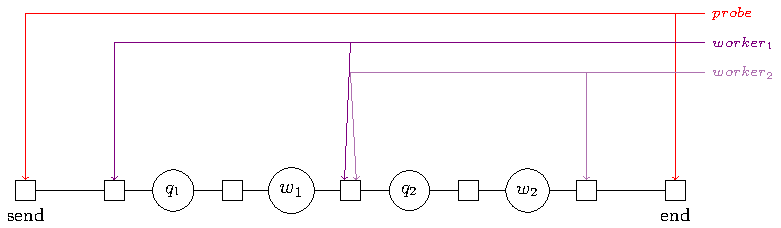
\includegraphics[scale=1.2, width=\textwidth]{tikz/mm1k.pdf} 
        \end{center}
        \caption{Outcome diagram of the M/M/1/K queue}
    \end{figure}
